\chapter{Case Study}
\label{ch:case_study}

\newcommand{\mysubparagraph}[1]{\subparagraph{#1}\mbox{}\\}

\section{Problem}

\subsection{Research Question}
\begin{itemize}
	\item In what ways do the tools correlate?
\end{itemize}

\section{Company F Information}

\subsection{Company F}
Company F \footnote{F is the first letter of the company's name} is a United States company which acts in the POS \footnote{Point Of Sales} area. With the development of some new products the company had a 400\% increase in the size of the development and QA departments resulting in the need for organizing better the development and release processes. In addition the increasing requests of new features in the company's systems requires a more efficient way in delivering them to the customers and also maintaining the quality of the products.

\subsection{Methodology F}
In general, company F does not follow a specific agile methodology, but rather a tailored mix of the most famous ones which suits the needs of each team. Methodology F, as we can name it, embraces the practices displayed in Table~\ref{table:methodologyF_practices} from the various agile methodologies, some of the them in bigger and some of them in a smaller extent. For identifying these methodologies the analysis made by \citet{koch2005agile} was used. The results were verified by the agile coach.

\begin{table} [H]
\caption{Practices embraced by methodology F}
\begin{tabular}{| p{2cm} | p{13cm}|}
    \hline
     \textbf{Method} & \textbf{Practice} \\ \hline
     \textbf{XP}  & \begin{inparaenum} [a\upshape)]
     				\item Small Releases \item Simple design \item Refactoring \item Collective ownership \item Continuous integration \item 40-hour week \item Coding standards
					\end{inparaenum}      \\ \hline
     \textbf{FDD}  & \begin{inparaenum} [a\upshape)]  \item Developing by feature \item Feature teams \item Regular build schedule \item Inspections \item Configuration management
     				  \end{inparaenum}\\ \hline
     \textbf{Lean} & \begin{inparaenum} [a\upshape)] \item Empower the team \item Build Integrity In \item Amplify learning \item Eliminate waste
     				 \end{inparaenum} \\ \hline
\end{tabular}
\label{table:methodologyF_practices}
\end{table}

\subsection{Products}
Company F has developed a few products which belong in the following four areas 
\begin{inparaenum} [a\upshape)]
\item desktop
\item mobile
\item cloud
\item platforms.
\end{inparaenum}
The names given are respectives to the name of the teams that develop them.

\begin{itemize}
\item Product A - A series of three mobile applications which offer services to stores or customers of stores.
\item Product B - A cloud application which offers services to product A and product D.
\item Product C - A platform used only by the company's employees. It supports services though which are necessary for product D.
\item Product D - It is the main product of the company which is mostly used. The rest of the products were developed in order to support it and expand its functionalities.

\end{itemize}

\subsection{Teams}
There are four development teams, each for a product of the company. Some of the teams have mixed members of developers and testers. In the Tables~\ref{table:teamA}, \ref{table:teamB}, \ref{table:teamC}, \ref{table:teamD}, one can see the structure of the teams. \\

\begin{table} [H]
  \RawFloats
 \begin{minipage}[b]{0.5\textwidth}
  \centering
    \caption{Team A - Profile} %Mobile
  \begin{tabular}{| p{3.3cm} | p{3cm}|}
    \hline
     \textbf{Team Size} & 7 \\ \hline
     \textbf{Roles}  & \begin{tabular}{@{}l@{}}Team Leader (1) \\ Developers (3) \\ Testers (3) \end{tabular} \\ \hline
  %   \textbf{Development Process}  & Method A \\ \hline
     \textbf{Area} & Mobile \\ \hline
     \textbf{Tools Used}  & \begin{tabular}{@{}l@{}}Perforce \\ Titanium \end{tabular}  \\ \hline
     \textbf{Iteration Length}  & 2-3 weeks \\ \hline
  \end{tabular}
  \label{table:teamA}
 \end{minipage} %
%
 \begin{minipage}[b]{.5\textwidth}
  \centering
    \caption{Team B - Profile} %Marketing
  \begin{tabular}{| p{3.3cm} | p{3cm}|}
    \hline
     \textbf{Team Size} & 6 \\ \hline
     \textbf{Roles}  & \begin{tabular}{@{}l@{}}Team Leader (1) \\ Developers (5) \\ Testers (1) \end{tabular} \\ \hline
    % \textbf{Development Process}  & Method B \\ \hline
     \textbf{Area} & Java \\ \hline
     \textbf{Tools Used}  & \begin{tabular}{@{}l@{}}Perforce \\ Eclipse IDE \end{tabular} \\ \hline
     \textbf{Iteration Length}  & 2-3 weeks \\ \hline
  \end{tabular}
  \label{table:teamB}
  \end{minipage} %
  
  \vspace{10 mm}
%
 \begin{minipage}[b]{.5\textwidth}
  \centering
    \caption{Team C - Profile} %Info
  \begin{tabular}{| p{3.3cm} | p{3cm}|}
    \hline
     \textbf{Team Size} & 4 \\ \hline
     \textbf{Roles}  & \begin{tabular}{@{}l@{}}Team Leader (1) \\ Developers (2) \\ Testers (1) \end{tabular} \\ \hline
 %    \textbf{Development Process}  & Method C \\ \hline
     \textbf{Area} & Java \\ \hline
     \textbf{Tools Used}  & \begin{tabular}{@{}l@{}}Perforce \\ Eclipse IDE \end{tabular}  \\ \hline
     \textbf{Iteration Length}  & 3-4 weeks \\ \hline
  \end{tabular}
  \label{table:teamC}
\end{minipage}%
%
 \begin{minipage}[b]{.5\textwidth}
  \centering
    \caption{Team D - Profile} %POS
  \begin{tabular}{| p{3.3cm} | p{3cm}|}
    \hline
     \textbf{Team Size} & 19 \\ \hline
     \textbf{Roles}  & \begin{tabular}{@{}l@{}}Team Leader (1) \\ Developers (10) \\ Testers (8) \end{tabular} \\ \hline
  %   \textbf{Development Process}  & Method D \\ \hline
     \textbf{Area} & Java \\ \hline
     \textbf{Tools Used}  & \begin{tabular}{@{}l@{}}Perforce \\ Eclipse IDE \end{tabular} \\ \hline
     \textbf{Iteration Length}  & 2-4 weeks \\ \hline
  \end{tabular}
  \label{table:teamD}
  \end{minipage}
\end{table}

%\section{OPS}
%
%\subsection{Introduction}
%In order to measure the adequacy, the capability and the effectiveness of methodology F, the described method by \citet{sventha_dissertation} was followed.
%
%\subsection{Adequacy Assessment}
%\label{subsec:adequacy_analysis}
%
%In order to assess the adequacy of methodology F a top-down traversal was used as it can be seen in Figure~\ref{ops_core}. For the analysis of each objective, principle and strategy the analysis of agile methodologies was followed based on \citet{koch2005agile}.
%
%Initially the objectives fulfilled by methodology F were identified. As one can see in Figure~\ref{fig:companyF_objectives} all five objectives instructed by the OPS Framework are followed.
%
%\begin{figure}[H]
%\centerline{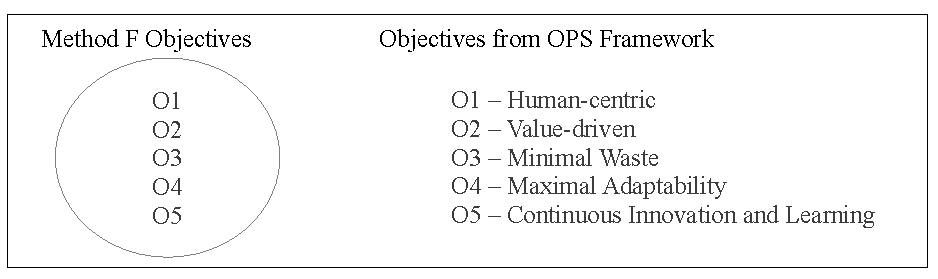
\includegraphics[scale=0.9]{include/case_study/fig/companyF_objectives.pdf}}
%\caption{Objectives identified in methodology F} 
%\label{fig:companyF_objectives}
%\end{figure}
%
%Based on the objectives and following the linkages from them, the principles were identified. As one can see in Figure~\ref{fig:companyF_objectives} methodology F does not follow the ``Frequent Reflection and Improvement" principle because the organization rarely does it re-examine the development process in order to improve it. %maybe justify why!
%It is worth mentioning that the ``Empowering teams of Motivated Individuals" principle is not entirely followed either, but it differs among the teams. Every team is built with motivated individuals, some to a more and some to a lesser extent. 
%
%\begin{figure}[H]
%\centerline{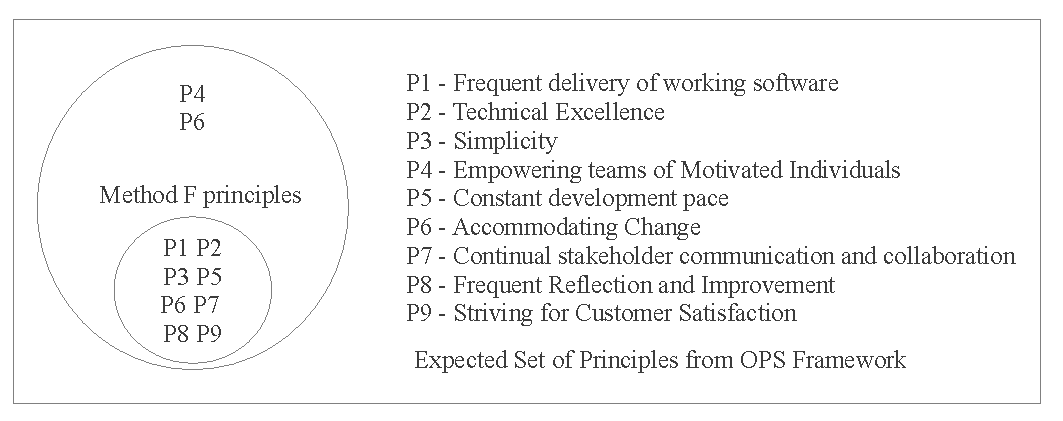
\includegraphics[scale=0.9]{include/case_study/fig/companyF_principles.pdf}}
%\caption{Principles identified in methodology F} 
%\label{fig:companyF_principles}
%\end{figure}
%
%Following the linkages from the principles the strategies for implementing them were identified. As it can be seen in Figure~\ref{fig:companyF_strategies} methodology F does not support 
%
%\begin{itemize}
%\item \textbf{Continuous feedback} - The organization does not have a defined process for getting a feedback from the customers of the company. From time to time the managers of the various departments of the company have personal conversations with the customers. If any issue arises, then they inform the development and QA departments in order to identify the problem and fix it.
%\item \textbf{Test-first development} - None of the team members writes tests before starting coding.
%\item \textbf{Constant velocity} - The organization does not measure the velocity of the teams. In general the pace of development and integration and deployment is based on the needs of the customers and the capability of the developer. No one has to finish a specific amount of work in each iteration. What is only wanted, is the functionality to be delivered when it is scheduled.
%\item \textbf{Retrospection} - Although there is a tendency to change this, the teams do not have a process for retrospection. The team members unconsciously consider that they are doing fine, unless a team leader or the manager of the department tells them the opposite.
%\end{itemize}
%
%\begin{figure}[H]
%\centerline{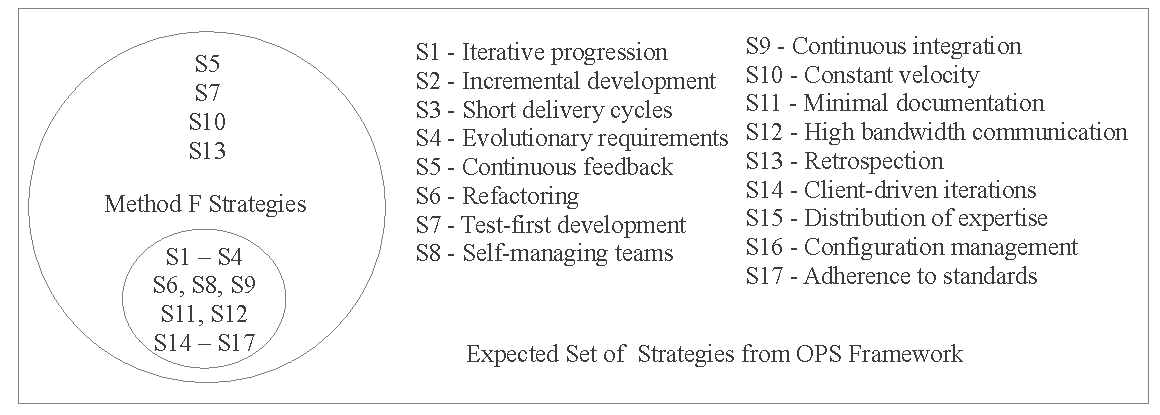
\includegraphics[scale=0.9]{include/case_study/fig/companyF_strategies.pdf}}
%\caption{Strategies identified in methodology F} 
%\label{fig:companyF_strategies}
%\end{figure}
%
%%Analyze more the adequacy
%Reflecting on the above analysis, we see that methodology F lacks four strategies which are important for its improvement. Without retrospection the team members do not always identify and discuss their mistakes, while without a well defined process for continuous feedback any issues that might arise may go unnoticed for quite some time. In total, methodology F is missing four strategies out of seventeen which is a lot.


\section{Methodology}
%need to change the intro
In order to see which of the OPS, PAM and TAA can better measure the agility of software development teams, the four teams in company F were used as a sample.

\subsection{Data Collection}

%maybe provide numbers for the demographics

\subsubsection{Surveys}
In order to collect the data an online survey was considered to be the best option since it could be easily answered by each subject and in addition this would assure no data loss. Google Drive \texttrademark \cite{google_drive} was selected to be the platform for collecting and preserving the data.

For each of the tools, four surveys were created for each team respectively. The collection lasted about one month, the surveys for each tool every ten days. First PAM was sent, then TAA and at last it was OPS.

Two subjects were requested to answer to the surveys first, in order to detect if there were any questions which could cause confusion, but also to see how much time is needed to fill in the surveys. Once the issues pointed out by the two subjects were fixed, the surveys were sent to the rest of the company's employees.

The links to the surveys were sent to the subjects early in the morning with an email, but they were asked to answer to them after lunch. The reasoning for this, is that at the beginning of the day the employees need to perform tasks which are usually important and time consuming and require to have clear thoughts and be on meetings. On the contrary, after lunch most of the employees try to relax by enjoying their coffee and discussing with each other. That time of the day was considered to be the best in order to ask them to spend 15-20 minutes and reply to the survey. The employees that belonged to more than one team, were asked a couple of days later to take the other survey in order to be more detached in their answers. Every question of the surveys was mandatory.

As it was mentioned in chapter~\ref{ch:related_work}, PAM focuses on the following agile practices:
\begin{inparaenum} [a\upshape)]
	\item Iteration Planning
	\item Iterative Development
	\item Continuous Integration And Testing
	\item Stand-Up Meetings
	\item Customer Access
	\item Customer Acceptance Tests
	\item Retrospectives
	\item Co-Location.
\end{inparaenum}
From these methodology F does not support \textit{Stand-Up Meetings} and \textit{Retrospectives} and as a result they were totally excluded from the surveys.

On the contrary, TAA focuses on the following agile practices/areas:
\begin{inparaenum} [a\upshape)]
	\item Product Ownership
	\item Release Planning and Tracking
	\item Iteration Planning and Tracking
	\item Team
	\item Testing Practices
	\item Development Practices/Infrastructure.
\end{inparaenum}
From the above practices, methodology F does not support \textit{Product Ownership}, since it implies that company F should practice Scrum, which it does not. Moreover, Scrum oriented questions from the rest of the practices/areas were removed as well. 

Finally, OPS focuses on the following strategies:
\begin{inparaenum} [a\upshape)]
	\item Iterative progression
	\item Incremental development
	\item Short delivery cycles
	\item Evolutionary requirements
	\item Continuous feedback
	\item Refactoring
	\item Test-first development
	\item Self-managing teams
	\item Continuous integration
	\item Constant velocity
	\item Minimal documentation
	\item High bandwidth communication
	\item Retrospection
	\item Client-driven iterations
	\item Distribution of expertise
	\item Configuration management
	\item Adherence to standards

\end{inparaenum}
From the above practices, methodology F does not support \textit{Continuous feedback}, \textit{Constant velocity} and \textit{Retrospection}.%(also check the analysis in section ~\ref{subsec:adequacy_analysis}

%About the questions of the agile practices/areas which were not included, they were all given a value of 1, the least possible value. 

As it was stated earlier, in subsection~\ref{subsec:ops}, OPS measures agility based on three aspects. Adequacy, Capability and Effectiveness. Effectiveness measurement focuses on how well a team implements agile methodologies. Since the rest of the tools focus on the same thing, it was decided only to use the survey from Effectiveness and not take into account about Adequacy and Capability.

For a more clear view on the questions contained in the surveys, one can take a look at Appendices~\ref{ch:effectiveness_hierarchy},~\ref{ch:pam} and~\ref{ch:team_agility_assessment}.

\subsubsection{Likert Scales}
The surveys for PAM TAA and OPS were on a Likert scale 1-7 (never-always). From PAM,  only the \textit{Co-location} practice had its Likert scale 1-5 (different time zones-same room) since its creators preferred it in this way. For the transforamtion of the results for this practice, formula~\eqref{eq:likert_transformation} \cite{likert_transformation} was used.  \begin{equation} \label{eq:likert_transformation} x_2 = (1.5 * x_1) - 0.5 \end{equation} 

\subsubsection{Demographics} % Have to fix this. Better add a table
The employees that were asked to answer to the surveys where all the members of the software development teams which consisted of software and quality assurance (QA) engineers. All of the participating employees have more than a year in the company, while most of them have more than five years of work experience in an agile environment. Employees which had been working for less than six months in the company were not asked since it was considered they were not fully aware of the company's procedures or they were not familiar enough with them. Although code review is practised, it was avoided to ask from the code reviewers to take the same survey for the same team from that perspective because it would not provide more value to the results and in addition it would tire them a lot.

%\begin{table} [H]
%	\caption{}
%	\label{}
%	\begin{tabular}{| c | c |}
%		Working experience in agile environment &
%		Working experience in company F &
%	\end{tabular}
%\end{table}

\subsection{Collected Data}
Each respondent replied to 176 questions in total. Initially, 34 surveys were expected to be filled in, but at end then 30 of them were since some employees preferred not to participate in the study.

\subsection{Data Analysis}
As it was mentioned earlier (if not, mention why and how) the data gathered from the survey were grouped by the practices covered by OPP and as a consequence OPS. From the 18 practices in total, four of them, \begin{inparaenum} [a\upshape)] \item Minimal or Just Enough Documentation \item Customer User Acceptance Testing \item Evolutionary Requirements \item Constant Velocity \end{inparaenum}, are covered only by one tool. The rest of the practices were covered by at least two of the tools.

Initially there was the thought to analyse the data for each team separately but this would create an extensive overhead. In addition, teamA has so few members that the results would be inadequate. As a result it was preferred to form the data sets for each practice based on the answers from all the teams.

Based on the analysis performed at chapter~\ref{ch:tools_completness} it is clear that OPS covers more agile practices/areas. As a result it was decided to use these practices in order to check the correlation of the tools. In Appendix~\ref{ch:mapping} one can see how the questions are group based on the OPS practices. The data sets consist of the answers which were sorted by team as stated above and have the same order in all practices (i.e. the nth answer in every practice is given by the same person).

For the analysis of the data the correlation method was selected as it has been used in other cases of tools comparisons \cite{jalali_angelis} \cite{Delestras2013}. The initial thought was to use ``Pearson product-moment correlation" as it is the one mostly used in statistics. 

The four practices mentioned above were discarded for using correlation, since there would not be any.

In order to use Pearson’s correlation there must hold four prerequisites
\begin{enumerate}
\item The two variables should be measured at the interval or ratio level
\item The variables should be approximately normally distributed
\item There needs to be a linear relationship between the two variables
\item There should be no significant outliers
\end{enumerate}

Since the data were collected by surveys using Likert scales, then prerequisite \#1 is satisfied, as the Likert scales can be considered both for interval or ratio level measurements, depending on the problem each time.

As far as the normal distribution is concerned, the Shapiro-Wilk test was selected as it appears to be the most powerful normality test according to a recent paper published by \citet{Razali}. In order for a distribution to be considered normal, the p-value must be greater than the alpha level so as not to reject the null hypothesis and consider that the data are normally distributed. The chosen alpha level was 0.05 as it is the most common one.

Out of the 42 normality checks (three for each of the 14 practices) only 17 concluded that the data are normally distributed. 

The low level of normally distributed data gave a strong indication that the Pearson’s correlation would not be the appropriate way to measure the tools' correlation. As a result it was preferred not to continue checking the last two prerequisites for Pearson’s correlation, but rather use ``Spearman’s rank correlation coefficient" which is for non-parametric data.

In order to use Spearman’s rank correlation coefficient two prerequisites must be satisfied
\begin{enumerate}
\item The two variables should be measured at the interval or ratio level
\item There needs to be a monotonic relationship between the two variables
\end{enumerate}

The first prerequisite was already covered above. In order to check for the monotonicity, plots were drawn between the results of each tool for all 14 practices. The plots surprisingly showed that only 8 out of 42 were monotonic, which does not allow to use Spearman’s correlation for the rest. The table~\ref{table:practices_spearman} summarizes the practices and the relationships in which Spearman's correlation can be used.

\begin{table} [H]
\caption{Pairs of tools for which Spearman's correlation can be used}
\label{table:practices_spearman}
\begin{tabular}{| c | c |}
\hline
\textbf{Practice} & \textbf{Tools Correlation} \\ \hline
Continuous Feedback & PAM - OPS \\ \hline
High Bandwidth Communication & \begin{tabular}{c} PAM - TAA \\ PAM - OPS \\ TAA - OPS \\ \end{tabular} \\ \hline
Client Driven Iterations &  PAM - OPS \\ \hline
Continuous Integration & PAM - TAA \\ \hline
Iterative and Incremental Development & PAM - OPS \\ \hline
Refactoring & PAM - TAA \\ \hline
\end{tabular}
\end{table}

The cells for which a correlation exists are coloured in green in order to distinguish from the rest. In Table~\ref{table:correlations_frequency} one can see that half of the correlations are between PAM and OPS. This corroborates that OPS has full coverage of PAM as seen in Table ~\ref{table:questions_coverage}. %maybe add in the Analysis - chapter 4

\begin{table} [H]
 \RawFloats %allows to have captions in all of the tables
 \begin{minipage}{.45\textwidth}
  \caption{Continuous Feedback Correlations}
  \label{table:cf_correlations}
   \begin{tabular}{| c | c | c | c |} \hline
   \multicolumn{4}{|c|}{\textbf{Continuous Feedback}}  \\ \hline
   & PAM & TAA & OPS \\ \hline
   PAM & 1.000 & NA & \cellcolor{green}0.459 \\ \hline
   TAA & NA & 1.000 & NA \\ \hline
   OPS & \cellcolor{green}0.459 & NA & 1.000 \\ \hline
  \end{tabular}
 \end{minipage}%
%
 \begin{minipage}{.45\textwidth}
  \centering
  \caption{Client Driven Iterations Correlations}
  \label{table:cdi_correlations}
  \begin{tabular}{| c | c | c | c |} \hline
  \multicolumn{4}{|c|}{\textbf{Client Driven Iterations}}  \\ \hline
   & PAM & TAA & OPS \\ \hline
  PAM & 1.000 & NA & \cellcolor{green}0.161 \\ \hline
  TAA & NA & 1.000 & NA \\ \hline
  OPS & \cellcolor{green}0.161 & NA & 1.000 \\ \hline
 \end{tabular}
 \end{minipage}%
 %
\end{table}


\begin{table} [H]
 \RawFloats %allows to have captions in all of the tables
 \begin{minipage}{.45\textwidth}
  \caption{High Bandwidth Communication Correlations}
  \label{table:hbc_correlations}
  \begin{tabular}{| c | c | c | c |} \hline
  \multicolumn{4}{|c|}{\textbf{High Bandwidth Communication}}  \\ \hline
  & PAM & TAA & OPS \\ \hline
  PAM & 1.000 & \cellcolor{green}0.322 & \cellcolor{green}-0.023 \\ \hline
  TAA & \cellcolor{green}0.322 & 1.000 & \cellcolor{green}0.237 \\ \hline
  OPS & \cellcolor{green}-0.023 & \cellcolor{green}0.237 & 1.000 \\ \hline
 \end{tabular}
 \end{minipage}%
%
 \begin{minipage}{.45\textwidth}
  \centering
  \caption{Refactoring Correlations}
  \label{table:ref_correlations}
  \begin{tabular}{| c | c | c | c |} \hline
  \multicolumn{4}{|c|}{\textbf{Refactoring}}  \\ \hline
   & PAM & TAA & OPS \\ \hline
   PAM & 1.000 & \cellcolor{green}0.097 & -0.050 \\ \hline
   TAA & \cellcolor{green}0.097 & 1.000 & 0.181 \\ \hline
   OPS & -0.050 & 0.181 & 1.000 \\ \hline
  \end{tabular}  
 \end{minipage}%
 %
\end{table}

\begin{table}
 \RawFloats %allows to have captions in all of the tables
 \begin{minipage}{.45\textwidth}
  \caption{Continuous Integration Correlations}
  \label{table:ci_correlations}
  \begin{tabular}{| c | c | c | c | } \hline
  \multicolumn{4}{|c|}{\textbf{Continuous Integration}}  \\ \hline
   & PAM & TAA & OPS \\ \hline
  PAM & 1.000 & 0.398 & \cellcolor{green}0.249 \\ \hline
  TAA & 0.398 & 1.000 & 0.115 \\ \hline
  OPS & \cellcolor{green}0.249 & 0.115 & 1.000 \\ \hline
 \end{tabular}
 \end{minipage}%
%
 \begin{minipage}{.45\textwidth}
  \centering
   \caption{Iterative and Incremental Development Correlations}
  \label{table:iid_correlations}
  \begin{tabular}{| c | c | c | c |} \hline
  \multicolumn{4}{|c|}{\textbf{Iterative and Incremental Development}}  \\ \hline
  & PAM & TAA & OPS \\ \hline
  PAM & 1.000 & 0.204 & \cellcolor{green}0.396 \\ \hline
  TAA & 0.204 & 1.000 & -0.228 \\ \hline
  OPS & \cellcolor{green}0.396 & -0.228 & 1.000 \\ \hline
 \end{tabular}
 \end{minipage}%
 %
\end{table}

\begin{table} [H]
	\caption{Frequency of correlation between tools}
	\label{table:correlations_frequency}
	\begin{tabular}{| c | c |} \hline
		\multicolumn{2}{|c|}{\textbf{Frequency}}  \\ \hline
		PAM-OPS & 4 \\ \hline
		PAM-TAA & 3 \\ \hline
		TAA-OPS & 1 \\ \hline
	\end{tabular}
\end{table}


The analysis of the data is presented in the next section.


%FIX VALUES FOR PAM
%
%In the Tables~\ref{table:pam_results} and~\ref{table:taa_results} one can see the average value of the team replies in every agile practice/area \footnote{The ones  marked with $^\ast$ are not included in the surveys}. All the answers were trimmed to two decimal points.
%
%\begin{table} [H]
%\caption{Perceptive Agile Measurement Results}
%\label{table:pam_results}
%\begin{tabular}{| c | c | c | c | c |}
%\hline
%  & \multicolumn{4}{c|}{\textbf{Team}} \\ \hline
%\textbf{Practice} & Mobile & Info & POS & Marketing \\ \hline
%Iteration Planning & 3.86 & 5 & 4.08 & 3.66 \\ \hline
%Iterative Development & 4.36 & 5.71 & 5.3 & 5.09 \\ \hline
%Continuous Integration And Testing & 4.28 & 3.7 & 4.29 & 4.2 \\ \hline
%Customer Access & 4.58 & 7 & 5.5 & 3.9 \\ \hline
%Customer Acceptance Tests & 3.4 & 3.4 & 3.83 & 1.64 \\ \hline
%Co-Location & 4.27 & 6.13 & 5.59 & 6.2 \\ \hline 
%Stand-Up Meetings$^\ast$ & 1 & 1 & 1 & 1 \\ \hline
%Retrospectives$^\ast$ & 1 & 1 & 1 & 1 \\ \hline
%\textbf{Total} & 3.47 & 4.12 & 3.82 & 3.53 \\ \hline
%\end{tabular}
%\end{table}
%
%\begin{table} [H]
%\caption{Team Agility Assessment Results}
%\label{table:taa_results}
%\begin{tabular}{| c | c | c | c | c |}
%\hline
%  & \multicolumn{4}{c|}{\textbf{Team}} \\ \hline
%\textbf{Agile Area} & Mobile & Info & POS & Marketing \\ \hline
%Release Planning and Tracking & 4.54 & 4.17 & 4.43 & 4.38 \\ \hline
%Iteration Planning and Tracking & 3.98 & 3.58 & 4.04 & 3.7 \\ \hline
%Team & 4.95 & 4.93 & 4.73 & 4.44 \\ \hline
%Testing Practices & 3.86 & 2.56 & 3.3 & 3.77 \\ \hline
%Development Practices/Infrastructure & 5.92 & 5.94 & 5.49 & 5.5 \\ \hline
%Product Ownership$^\ast$ & 1 & 1 & 1 & 1 \\ \hline 
%\textbf{Total} & 4.04 & 3.7 & 3.83 & 3.8 \\ \hline
%\end{tabular}
%\end{table}


\section{Correlations Analysis}

In \textit{Continuous Feedback} PAM and OPS have a moderate positive correlation of 0.459. Both tools focus on getting feedback from the customer, while OPS also checks whether the product is developed according to the customer's needs and expectations.

In \textit{Client-Driven Iterations} PAM and OPS have a low positive correlation of 0.161. Both tools check for  the possibility of the requirements having been prioritized by the customer. %Add more

\section{Discussion}

\subsection{Introduction}
As it was seen by the reader the correlation of only a few of the practices can be examined. In this section the reasons for this will be presented and discussed.

\subsection{Reasons for results}


\subsubsection{The tools measure a practice in the same way}
Tools that claim to measure agility in the same way are expected to do so. Unfortunately this does not imply that their correlation can be calculated. The figure~\ref{fig:scm_plot} made it very clear why. All the answers from all the teams and for TAA and OPS were the same. Both tools had a unique question about using a version control management system, which stands true for company F for anything that has to do with code changes. The designed plots only had one spot which means the correlation among the tools is not possible to calculate due to lack of variation in the results. Such an occurrence shows that correlation techniques can be defective when checking tools which manage to measure the same thing to the same extent.

\subsubsection{The tools have few or no questions for measuring a practice}
Another reason for not being able to calculate the correlation of the tools is that they cover slightly or not even at all some of the practices. An example of this, is the \textit{Smaller and Frequent Product Releases} practice. OPS has four questions for it, while on the other hand PAM and TAA have a single one each. Furthermore, \textit{Appropriate Distribution of Expertise} is not covered at all by PAM while it is by the rest of the tools. In case the single question gets a low score this will affect the effectiveness of the tool. On the contrary, multiple questions can cover more completely the practice by examining more factors that affect it. Apart from measuring a practice more precisely this also has the benefit that even if a question gets a low score, the rest of them are candidates for getting a higher one. The issue is worse if a practice is not covered at all. Unfortunately this phenomenon does not allow to equally check all the tools giving a respected superiority to the ones that take the practice into consideration and even more to the ones that do that to an extended degree.

\subsubsection{The tools measure the same practice differently}
Something very interesting that came up during the data analysis was that the tools although they cover the same practices they do it in different ways, leading in different results. An example of this is the practice of \textit{Refactoring} ~\ref{fig:ref_plot}. PAM checks whether there are enough unit tests and automated system tests to allow the safe code refactoring. In case of course unit/system tests are not developed by a team, then the respondents will give low scores to the question, as the team members in company F did. Nevertheless, this does not mean that the team never refactors the software or it does it with bad results. All teams in company F choose to refactor when it adds value to the system, but the level of unit tests is very low and they exist only for specific teams. On the other hand, TAA and OPS check how often do the teams refactor among other factors which allows to better evaluate the practice of refactoring. Considering the above, PAM seems to fail to measure the \textit{Refactoring}.

\subsubsection{The tools measure the same practice in opposite questions}
The \textit{Continuous Integration} practice has a unique paradox among TAA, PAM and OPS. The first two tools have a question about the members of the team having synced to the latest code, while OPS checks for the exact opposite. According to \citet{sventha_dissertation} it is preferable for the teams not to share the same code in order to measure the practice. It is quite doubtful though how correct can this question be, since the \textit{Continuous Integration} requires for frequent submits from the developers and thus the rest of the team will also have a local version of the code.

\subsubsection{Questions phrasing}
Although the tools might cover the same areas for each practice, the results could differ because of how a question is structured. An example of this is the \textit{Test Driven Development} practice. Both TAA and PAM ask about automated code coverage, while OPS just asks about the existence of code coverage. Furthermore, TAA focuses on 100\% automation while PAM doesn’t. Thus, if a team has code coverage but it is not automated, then the score to the respective question should be low. In case of TAA if it is fully automated it should be even lower. It is evident that the more specific a question is, the more its answer will differ resulting in possible low scores.

\subsubsection{How people perceive agility}
Although the concept of agility is not new, people don’t seem to fully understand it. This is actually the reason for having so many tools in the field trying to measure how agile are the teams or the methodologies used by them. Teams implement agile methodologies differently and researchers create different measurement tools. There are numerous definitions about what agility is \cite{Kidd, NagelDove, Kara, Ramesh}, and each of the tools creator adopt or adapt one to their needs. Their only common basis is the agile manifesto \cite{beck2001agile} and its twelve principles \cite{agile_principles} which are (and should be considered as) a compass for the agile practitioners. Nevertheless, they are not enough resulting in the saturation of the field. Moreover, \citet{conboy_fitzgerald} state that the Agile Manifesto principles do not provide practical understanding of the concept of Agility. Consequently, all the aforementioned reasons for the survey results as stated above, are driven by the fact how people perceive agility. The word people refers to the tool creators and tool users.

The questions in the surveys were all based on how their creators perceived the agile concept which as explained above it is vague. As the reader has seen in previous chapters PAM, TAA and OPS focus on some common areas/practices, such as  \textit{Smaller and Frequent Product Releases} and \textit{High-Bandwidth Communication} while many are different. None of the \citet{sventha_dissertation}, \citet{pam}, \citet{Leffingwell} claimed of course to have created the most complete measurement tool, but still this leads to the oxymore that tools created by specialists to measure the agility of software development tools, they actually do it differently.

Considering that the researchers and specialists in the agile field perceive differently the concept of agility it would be naive to say that teams don’t do the same. The answers in surveys are subjective and people answer them depending on how they understand them. This is also corroborated, by the fact that although a team works at the same room and follows the same processes for weeks it is rather unlikely if its members will have the same understanding what it means for them a retrospection or a releasing planning meeting.